\documentclass{article} % For LaTeX2e
\usepackage{iclr2018_conference,times}
\usepackage{hyperref}
\usepackage{url}
\usepackage{graphicx}
\usepackage{amssymb}
\usepackage{amsmath}
\usepackage{caption}
\usepackage{subcaption}
\usepackage{algorithm}
\usepackage{algpseudocode}
\usepackage{listings}



\title{Practical Investigation into Safe Reinforcement Learning with Autonomous Drive}

\author{Tao Sun \\
taosun.victor@gmail.com \\
SanDisk, a Western Digital Brand  
}

%\newcommand{\fix}{\marginpar{FIX}}
%\newcommand{\new}{\marginpar{NEW}}

\iclrfinalcopy % Uncomment for camera-ready version, but NOT for submission.

\begin{document}


\maketitle

\begin{abstract}
Reinforcement learning is a popular and powerful tool to learn optimal policies concerning games and control systems. However, in order to find the optimal policy, most reinforcement learning algorithms would do a few trial-and-error explorations at the beginning of the learning stage. Concerning real world control systems, these trial-and-error explorations might violate the safety constraints and cause damages to the system. This problem could be more serious when it comes to safety-critical applications, such as autonomous drive. In this project, we try to implement a recently proposed practical approach to help the autonomous drive system learn its optimal policy safely. Specifically, our goal is to ensure the system's explorations to stay within the safety constraints during the overall learning stage. We present the implementation and corresponding results, together with some discussions.
\end{abstract}

%==========================================================================================================
\section{Introduction}
In the past few years, reinforcement learning (RL) has been explored in many environments, such as video games \cite{mnih2015human}, Go games \cite{silver2016mastering}, robotic design \cite{kober2013reinforcement} and so on. However, the RL algorithms normally provide an optimal policy only in the long term, and the immediate actions proposed might be unsafe and break the safety constraints. The unsafe actions might produce harmful results to the system. This is more serious when it comes to safety-critical areas. Thus safety for RL has been an open question in industrial applications.

Autonomous driving system falls into such kind of safety-critical area. Consider a self-driving car learning to drive with certain RL algorithms. At the very beginning of the learning stage, the RL algorithms might propose some unsafe actions based upon currently learned policy. Of course the unsatisfactory reward from such unsafe actions would help to improve the learned policy, however, the proposed action has to be applied in order for the system to take the negative feedback from the reward. Such unsafe actions might bring serious results, such as car accidents. Here is the dilemma, the RL algorithm has to explore the unsafe action space to improve its policy, but serious outcomes might come when such actions are carried out. Such situation is very common in real-world applications. Despite the powerful impact of RL algorithm, safety ensurance is an important problem to address. 

In general, several works have been published to discuss the safety guarantees in RL applications. \cite{berkenkamp2017safe} describes theoreical conditions under which safe explorations could be guaranteed for certain control systems. Some prior knowledge about the physical system and certain mathematical conditions should be satisfied. Basically a physical model describing the deterministic part of the dynamics should be known, above that a Lyapunov function should be identified for policy attraction region under certain Lipschitz continuity conditions. Despite the results revealed by mathematical descriptions, sometimes a physical model is hard to find for complicated systems. Another example is \cite{achiam2017constrained}, in which a modified trust-region policy gradient method is used to solve the constrained policy optimization problem. In each iteration, the optimization algorithm projects the the policy to a safe feasibility set. The safety constraints are met in expectation, not every iteration, which would still cause some problems. 

A more recent work \cite{dalal2018safe} proposes a much simpler and practical approach. In this approach, the safety signal is defined as a measure concerning the safety constraints. Some prior sampled data regarding state transition, actions taken and corresponding safety signals are dumped and used to train a model called "safety layer". The safety layer is used to predict the resultant safety signals based on the current state and proposed action, to decide whether the action should be revised before being carried out. The approach is pretty straightforward and easy to implement. In the paper, the authors claim that the approach solves step-wise safety problem. However, their examples presented are not really complicated, with low dimensional state space and simple environment. 

This triggers the current project, whether the approach proposed by \cite{dalal2018safe} could be applied to more complicated applications, specifically, autonomous drive, to ensure step-wise safety during reinforcement learning process. It is well known that autonomous drive is a complicated application with complex environment and high dimensional state space (image). We would like to adopt the proposed safety-layer approach to autonomous drive application, to see how it works.

%===================================================================================================
\section{Autonomous Drive with Reinforcement Learning}
Autonomous drive has been a popular yet challeging topic today. Despite the fact that many efficient RL algorithms has been proposed, their applications to autonomous drive still suffer from compliated system setup and lack of powerful enough hardwares. Recently $Wayve.ai$ introduces a method to train a self-driving car both in simulations and in real world \cite{kendall2018learning}. They deploy the method with the input state as a single image taken by the front camera on the car, and the output action from the policy learned by RL algorithms. This is the first practical implementation regarding RL applied to drive a real car. The method could let the car learn to drive in one day. The major point concerning algorithms is that they extract the features from the input image to represent the state with a variational auto-encoder (VAE). The representation from the VAE has much lower dimension than the original input image, so that the corresponding neural networks have smaller sizes and thus, fewer parameters to tune. The light-weighted neural network is relatively easy to train compared with traditional approaches of heavy-weighted neural networks. The schematic view of the above statement is as Figure 1.

\begin{figure}[!htb]
  \centering
  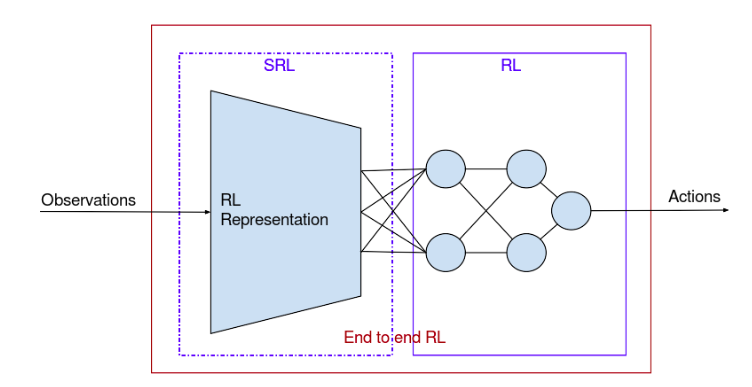
\includegraphics[width=0.7\linewidth]{fig1_srl.png}
  \caption{Extracting features from observations with state representation learning (SRL), then feeding the extracted features to reinforcement learning (RL) algorithms. The SRL used in this project is a VAE. Figure adapted from \cite{drive-smoothly-in-minutes}}
\end{figure}

A practical implementation of Wayve.ai's approach \cite{kendall2018learning} could be found as \cite{drive-smoothly-in-minutes}. In the implementation, the donkeyCar simulator \cite{donkeyCar-simulator} is used as the environment for autonomous drive. The VAE is trained based on the extracted images from the front camera of the toy car. The implementation provides several RL algorithms to experiment with: PPO2 \cite{schulman2017proximal}, DDPG \cite{lillicrap2015continuous} and SAC \cite{haarnoja2018soft}. The reward function is defined as in Equation 1, with $w_1$ and $w_2$ as predefined parameters. Basically the algorithm get small positive reward when traveling on the lane, and get large negative punishment when traveling off the lane. This reward would help the algorithm to improve its learned policy based on positive and negative feedbacks. With the help of VAE and RL algorithms, the toy car learns to drive in a few minutes.

\begin{equation}
reward = \begin{cases}
          -10 - w_1 \times throttle &\text{when off the lane}\\
          +1 + w_2 \times throttle  &\text{when on the lane}
         \end{cases}
\end{equation}

At the initial stage of training, several unsafe actions are observed, as shown in Figure 2. The RL algorithms needs to perform several unsatisfactory actions to get negative reward, before it could improve its policy to a proper state. These unsafe actions at the initial stage, however, are not desired. That's why we would like to explore ensuring safety during RL process.

\begin{figure}[ht]
\centering
\begin{subfigure}[b]{0.45\textwidth}
\centering
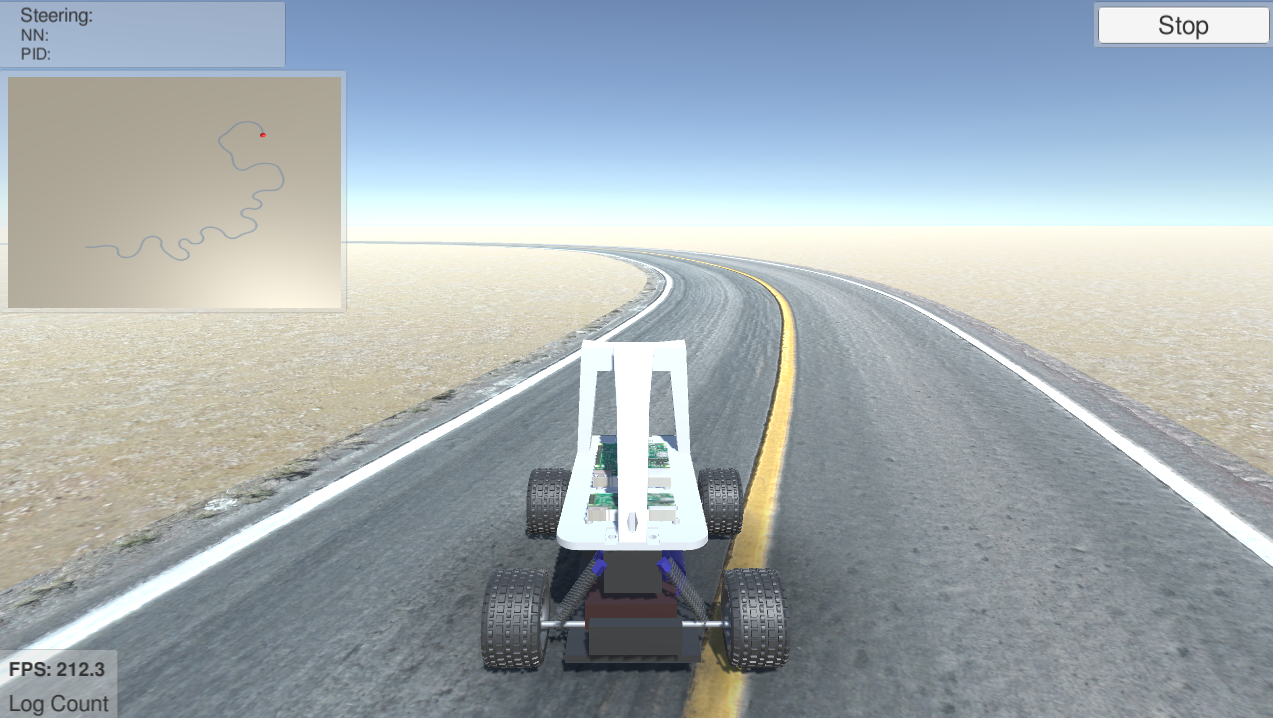
\includegraphics[width=\textwidth]{fig2a_left_cross.png}
\caption{}
\label{fig:gull}
\end{subfigure}%
\begin{subfigure}[b]{0.45\textwidth}
\centering
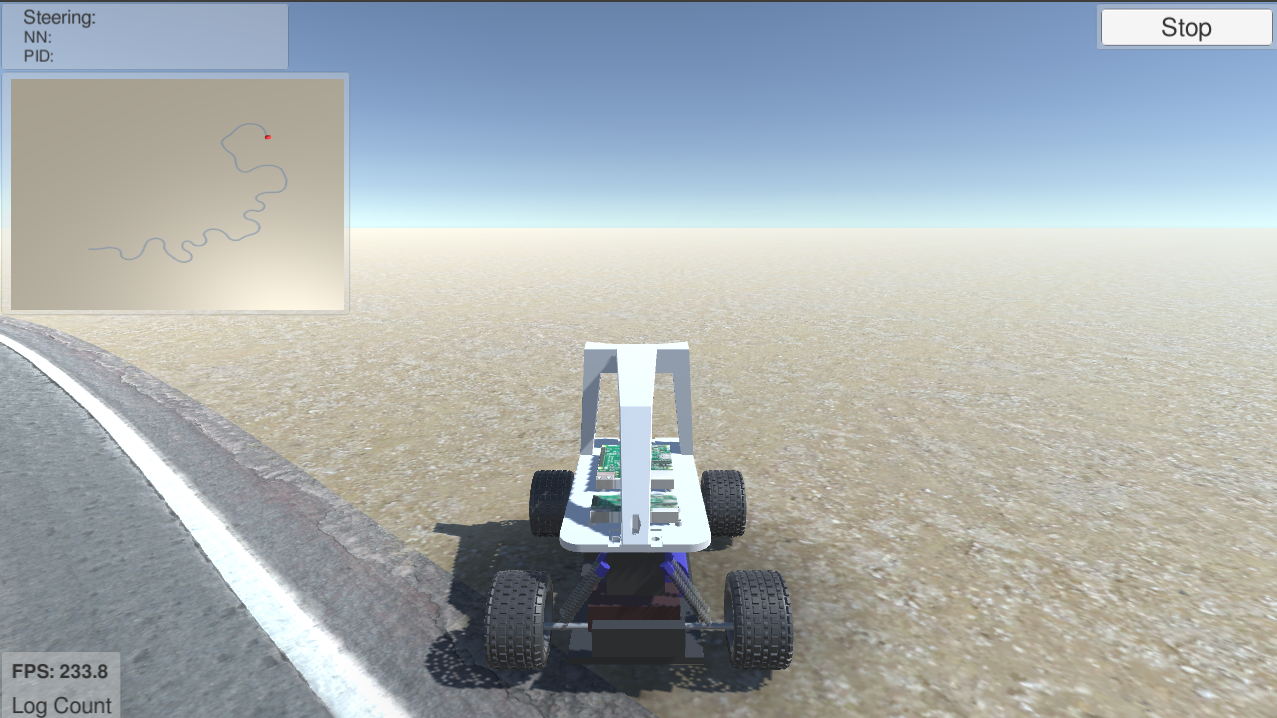
\includegraphics[width=\textwidth]{fig2b_right_cross.png}
\caption{}
\label{fig:gull}
\end{subfigure}%
\caption{Unsafe actions taken during training process. (a) Left cross out of the lane. (b) Right cross out of the lane.}
\end{figure}


%============================================================================================================
\section{Safety Layer method}
As stated in the Introduction section, \cite{dalal2018safe} proposed the safety layer method. The method first defines the so-called "safety signal" as the physical quantity indicating safety critical measurement that must stay within some constraints. For example in autonomous drive application, the safety signal could be defined as the maximum deviation of the car traveling outside the lane. 

The representations defined concerning the specific application in this project is as the following. The tuple to describe the problem is $(S, A, R, \gamma, C, \theta)$. $S$ is the state space, here is the extracted features from the VAE. $A$ is the action space as \textit{(steering angle, throttle)}. $R$ is the reward function, defined as Equation 1. $\gamma \in (0, 1)$ is the discount factor. $C=\{c: S \times A \rightarrow \mathbb{R}, c < C_{critical} \}$ is the safety constraint. Here $c$ represents the safety signal, and is defined as \textbf{the car's maximum deviation off the lane}. $C_{critical}$ is the corresponding constrain criteria that must be satisfied. The last one $\theta$ is the parameters representing the policy. The problem could be stated as, the RL algorithm learns a policy $\theta$ that takes input from state space $S$ and produces corresponding action as of $A$, then gets the reward as of $R$. At each step during learning, the safety constrain $C$ must be satisfied.

\begin{equation}
\begin{aligned}
\min_{\theta} \quad & \mathbb{E}(\sum_{t=0}^\infty \gamma^t R(s_t, \mu_{\theta}(s_t)) )\\
\textrm{s.t.} \quad & c(s_t) \leq C_{critical}\\
\end{aligned}
\end{equation}

Directly solving Equation 2 is very difficult, since the physical model governing the mapping between the safety signal and state/action pair is generally unknown. The method proposes to use a linear approximation to represent the safety signal.

\begin{equation}
\begin{aligned}
c(s') \approx c(s) + g(s, w)^\intercal a
\end{aligned}
\end{equation}

where $g(s, w)$ is a neural network takes $s$ as input and produces an output as a vector with the same dimention as $a$. The neural network $g(s, w)$ needs to be trained in advance, requiring sampling of safety signal transitions and corresponding states/actions pairs. Imaging we have a set of samples $D = \{(s_j, a_j, s_j')\}$, then the neural network could be trained as

\begin{equation}
arg \min_{w} \quad \sum_{(s, a, s')\in D} (c_i(s') - (c_i(s) + g(s, w)^\intercal a))^2\\
\end{equation}

Then we could add a safety layer to the RL algorithm. Basically the actions produced by the RL algorithm are screened by the safety layer to satisfy the constraints. The process is shown as Figure 3.

\begin{figure}[!htb]
  \centering
  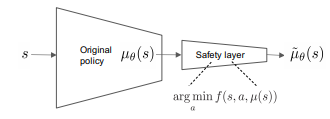
\includegraphics[width=0.5\linewidth]{fig3_scheme.png}
  \caption{A safety layer added after the RL policy layer. The figure is adapted from \cite{dalal2018safe}.}
\end{figure}

Now Equation 3 becomes the following form. Obviously a pretrained safety layer has been added on top of the RL policy layer, so that each time the proposed action produced by the RL algorithm would be revised by the safety layer. As a result, corresponding constraints could be satisfied.

\begin{equation}
\begin{aligned}
arg \min_{a} \quad & \frac{1}{2} |a - \mu_{\theta}(s)|^2\\
\textrm{s.t.} \quad & c(s) + g(s, w)^\intercal a \leq C_{critical}\\
\end{aligned}
\end{equation}

A close form solution exists for the constrained optimization problem presented in Equation 5 (thanks for the materials learned from ECE 490!). The close form solution is presented as the following.

$$\lambda_p = \frac{g(s, w)^\intercal \mu_{\theta}(s) + c(s) - C_{critical}}{g(s,w)^\intercal g(s,w)}$$

\begin{equation}
\lambda^{*} = \begin{cases}
           \lambda_p & \text{when $\lambda_p > 0 $} \\
           0         & \text{when $\lambda_p \leq 0$}
         \end{cases}
\end{equation}

$$a^* = \mu_{\theta}(s) - \lambda^* g(s, w)$$

Equation 6 is basically a linear projection of the originally proposed action to the safe hyperplane. The method is pretty easy to be implemented. In the paper \cite{dalal2018safe}, the authors have tried several easy examples to show that the above proposed method works so that there are zero safety violations. However, those examples are easy ones, with low dimension state space and simple environment. When it comes to the autonomous drive, the cases become more complicated concerning state space and environment. We would implement this method to autonomous drive simulations to see how it works.

%=======================================================================================================
\section{Implementation}
In this section, we implement the method from \cite{dalal2018safe} applied to autonomous drive system with a donkey car simulator. We have tried two examples, with the first example to be a simple environment and the second one to be a complicated environment. The method is tested on both with results presented.

\subsection{Simple Environment}
The first example is a simple environment, as shown from Figure 4. The lane is straight at most parts, with only several smooth turns from time to time. The environment, front camera image and VAE image are shown in the figure. We could see the VAE image could reveal the major features from the camera image. Our procedure for the RL algorithm training is shown as Algorithm 1.

\begin{figure}[ht]
\centering
\begin{subfigure}[b]{0.4\textwidth}
\centering
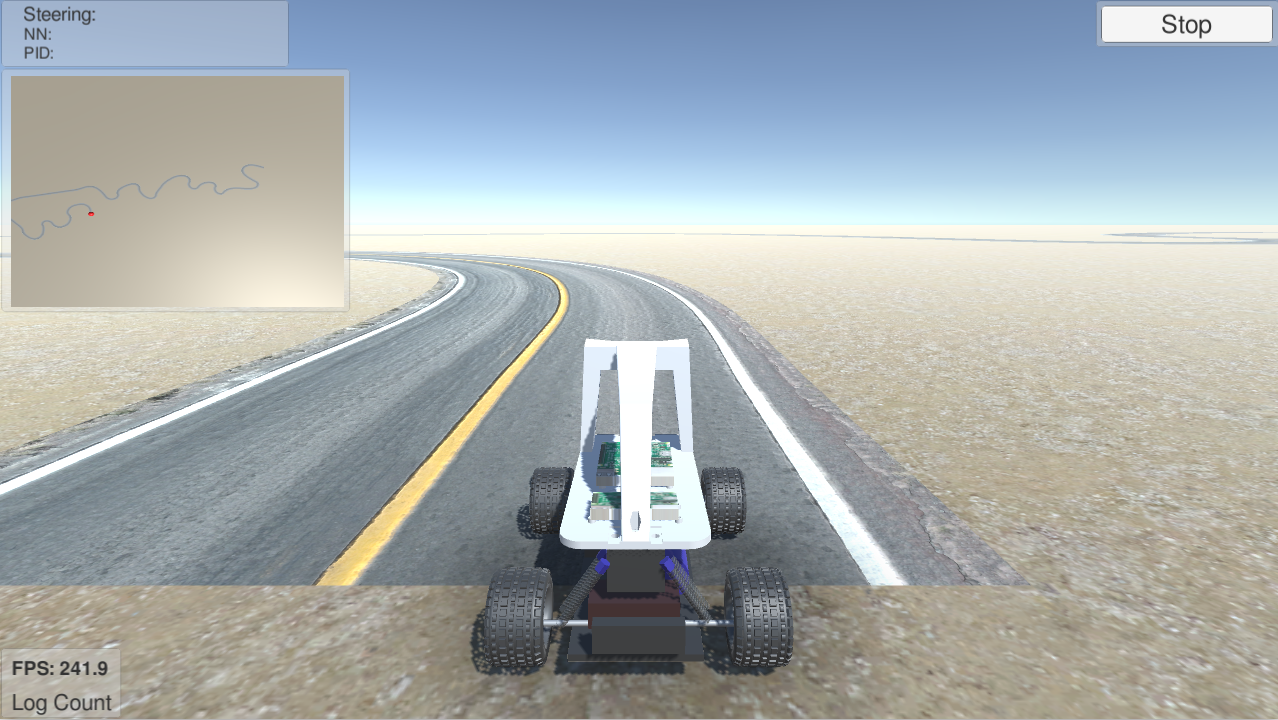
\includegraphics[width=\textwidth]{fig4a_simple_env.png}
\caption{Environment}
\label{fig:gull}
\end{subfigure}%
\begin{subfigure}[b]{0.45\textwidth}
\centering
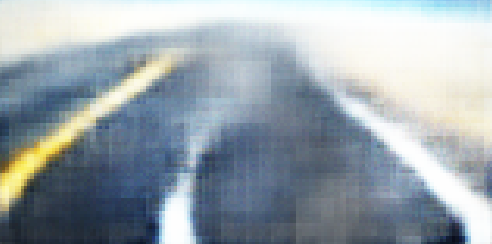
\includegraphics[width=\textwidth]{fig4c_vae.png}
\caption{VAE image}
\label{fig:gull}
\end{subfigure}%

\begin{subfigure}[b]{0.35\textwidth}
\centering

\includegraphics[width=\textwidth]{fig4b_camera.jpg}
\caption{Camera image}
\label{fig:gull}
\end{subfigure}%
\caption{First example, a simple environment. (a) Schematic view of the environment. (b) Image input from VAE, a compressed feature. (c) Image input from the front camera.}
\end{figure}

\begin{algorithm}[ht]
\caption{The Safety Layer with Linear Approximation}\label{euclid}
\begin{algorithmic}
\State{\textbf{Input}: donkey car simulator}
\State{Step 1}
    \State{$\quad\quad$Collect data tuples by random sampling:}
    \State{$\quad\quad$\{$c$: safety signal,}
    \State{$\quad\quad$ $s$: state (VAE image),}
    \State{$\quad\quad$ $a$: action (steering angle / throttle),}
    \State{$\quad\quad$ $c'$: new safety signal\}}
\State{Step 2}
    \State{$\quad\quad$Construct a neural network as the safety layer $g(s, w)$}
    \State{$\quad\quad$Train the safety layer according to Equation 4 with Gradient Descent}
\State{Step 3}
    \For{\text{step $\in$ (1, learning steps)}}
    \State{$\quad$Propose the initial action $\mu$ with the input state $s$ based on current RL policy}
    \State{$\quad$Correct $\mu$ according to Equation 6 to get action $\mu'$}
    \State{$\quad$Carry out action $\mu'$ to obtain the next state and reward}
    \State{$\quad$Update the policy according to the RL algorithm}
    \EndFor
\end{algorithmic}
\end{algorithm}

Here we collect the data tuples with random sampling and several partially trained models, in order to cover the major properties of the environment. For the safety layer we constructed a neural network with 2 fully connected hidden layers, with the first layer having 64 neurons and the second layer having 16 neurons. For the RL algorithms, we choose SAC algorithm \cite{haarnoja2018soft}. We run the learning process (starting from a barely trained model) without and with the safety layer, and try to compare the outcomes of these two. The results are shown in Figure 5.

\begin{figure}[ht]
\centering
\begin{subfigure}[b]{0.45\textwidth}
\centering
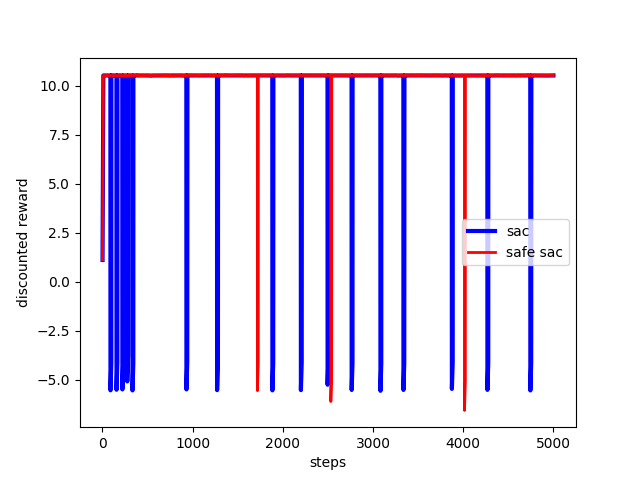
\includegraphics[width=\textwidth]{fig5a_reward.png}
\caption{}
\label{fig:gull}
\end{subfigure}%
\begin{subfigure}[b]{0.45\textwidth}
\centering
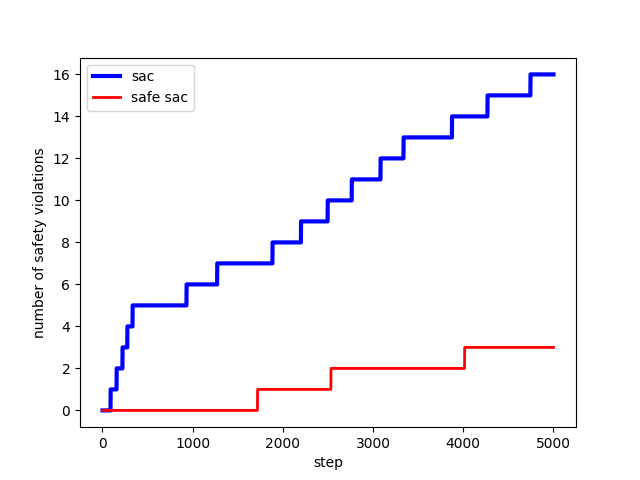
\includegraphics[width=\textwidth]{fig5b_violation.png}
\caption{}
\label{fig:gull}
\end{subfigure}%

\begin{subfigure}[b]{0.45\textwidth}
\centering
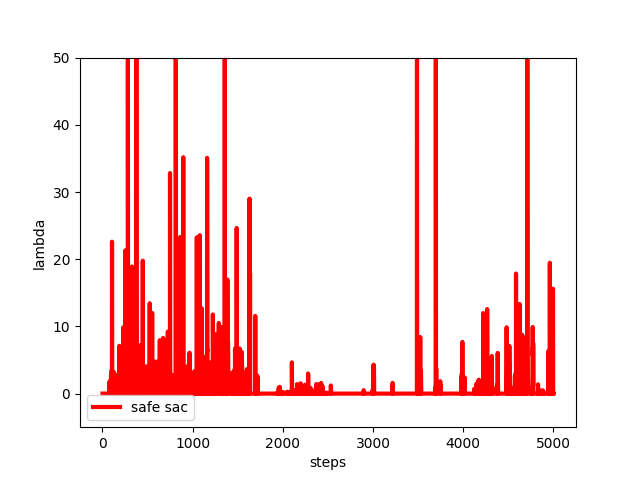
\includegraphics[width=\textwidth]{fig5c_lambda.png}
\caption{}
\label{fig:gull}
\end{subfigure}%
\caption{Comparison of the RL training process with/without safety layer. (a) Discounted reward. (b) Number of violations. (c) the value of $\lambda$, applied to safety layer method.}
\end{figure}
 
From Figure 5 we could obviously see that without safety layer, there are a number of safety violations at the training process. Also Figure 5b reveals that for the case without the safety layer, the safety violations are pretty common at the early stage. With the learning process going on, the safety violations are not so common any more, and would appear after many steps. It is reasonable to predict that after many steps of training, the policy is improved and there will be no more safety violations. For the case with safety layer, we could see that for 5000 steps of training, the number of safety violations is much smaller than the case without the safety layer. Moreover, at the very beginning of the training stage, there are no safety violations. Until at the middle and later stage, there are some safety violations happen. This reveals the fact that the safety layer do help to prevent safety violations at the early learning stage, and in general it ensures the safety. The safety violations appearing at the later time might be caused by not enough sampling of the state, since the lane is very long and the environment varies to some extent. For the case with the safety layer, the value of $\lambda$ evolving with training steps is showin in Figure 5c. We could see that at the initial learning stage, the value of $\lambda$ is pretty large, showing the originally proposed action from the partially trained policy would severly violate the safety constraint, and the safety layer does spend effort in bringing the car back. In the middle of the training process, the value of $\lambda$ is very small, showing the RL algorithm has updated its polity to a satisfactory state so that there are fewer safety violations. Then in the later part of the learning process, the value of $\lambda$ goes up again, showing the environment is varying.

Two videos are available for the RL training process without/with the safety layer \cite{safe-RL-video1}, \cite{safe-RL-video2}. From the videos, it is very clear that for the training process with the safety layer, each time when the car is about to violate the safety constraint (gets off the lane), the safety layer will simply push it back to the track. As a contrast, for the training process without the safety layer, there is no such luck. It will gets off the track from time to time.

The paper proposing the method \cite{dalal2018safe} shows that in the two example games, they achieve zero safety violations with the help of the safety layer. In our current case concerning autonomous drive system, since the environment is a lot more complicated, the safety layer could only confine the violation to some extent. But in general it works to reduce the number of safety violations.

%===============================================================================
\subsection{Complicated Environment}
Next we try a more complicated environment. The environment is shown in Figure 6. There are a number of continuous sharp turns on the way, and barely any simple straightforward paths exist. Also there are lots of obstacles on the road, making the environment more challenging. For the training stage of the safety layer, simple random sampling might not be able to capture the complicated environment. Together with the random sampling, we also adopt a trained model to drive the car along the road for a very long time (even the trained model violates the safety constraints for several times). The collected data are combined together to train the safety layer.

\begin{figure}[ht]
\centering
\begin{subfigure}[b]{0.45\textwidth}
\centering
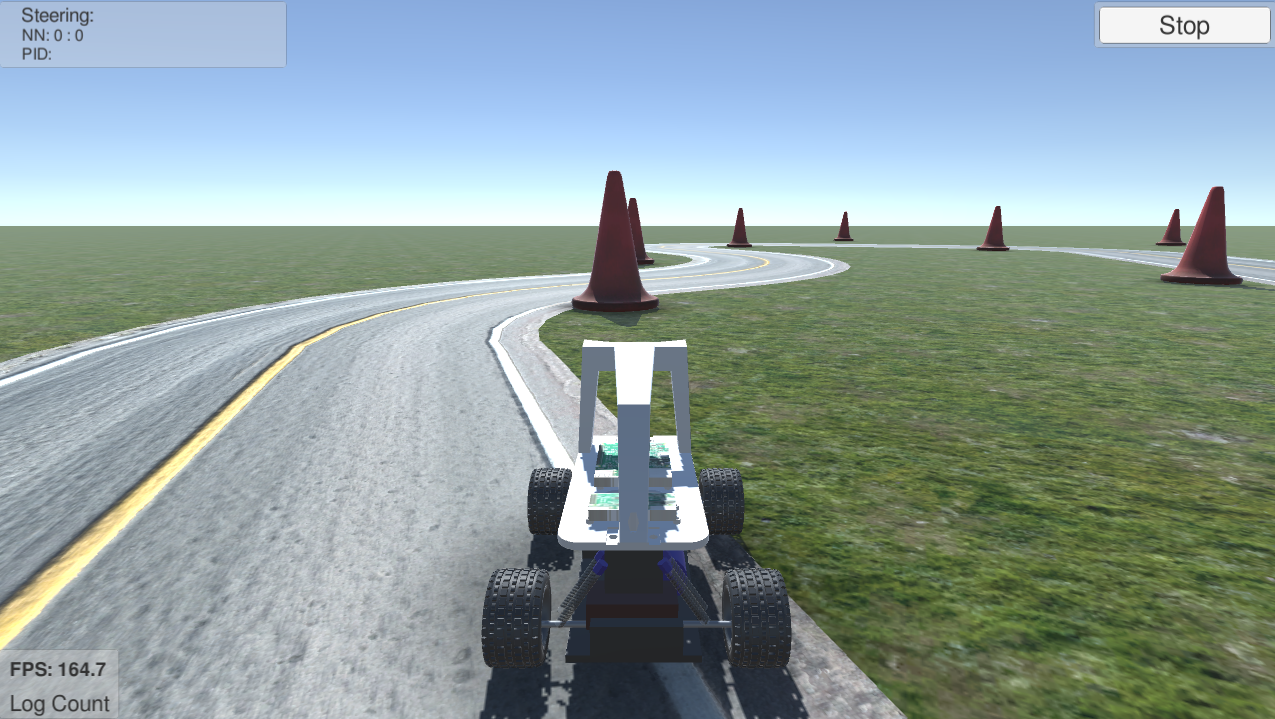
\includegraphics[width=\textwidth]{fig6a_complex_env.png}
\caption{Environment}
\label{fig:gull}
\end{subfigure}%
\begin{subfigure}[b]{0.34\textwidth}
\centering
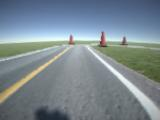
\includegraphics[width=\textwidth]{fig6b_camera.jpg}
\caption{Camera image}
\label{fig:gull}
\end{subfigure}%
\caption{Second example, a complicated environment. (a) Schematic view of the environment. (b) Image input from the front camera.}
\end{figure}

The results for the RL training process without/with safety layer (start from a barely trained model) under linear approximation is shown in Figure 7. We could see that even with the safety layer enabled, there are still many safety violations during the RL training stage, although the violations are slightly fewer than the case without the safety layer. For this complicated environment, we see that the safety layer does not provide very good result concerning eliminating the safety violations. The reason could be that, in this complicated environment, there are lots of sharp turns (as in Figure 7c). When the car is about to violate the left boundary, the safety layer would push it back to the center of the track. However, since this is a sharp turn, the car is approaching the right boundary of the track very quickly. When it is about to violate the right boundary, although the safety layer still tries to push it backward, the effect is no longer enough to prevent the car from getting off the lane. This shows the drawback of the current safety layer method. The corresponding video showing this could be found at \cite{safe-RL-video3}.

\begin{figure}[ht]
\centering
\begin{subfigure}[b]{0.45\textwidth}
\centering
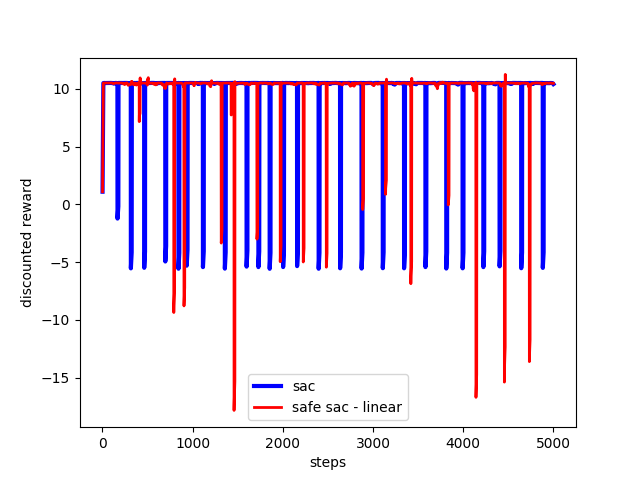
\includegraphics[width=\textwidth]{fig7a_l_reward.png}
\caption{}
\label{fig:gull}
\end{subfigure}%
\begin{subfigure}[b]{0.45\textwidth}
\centering
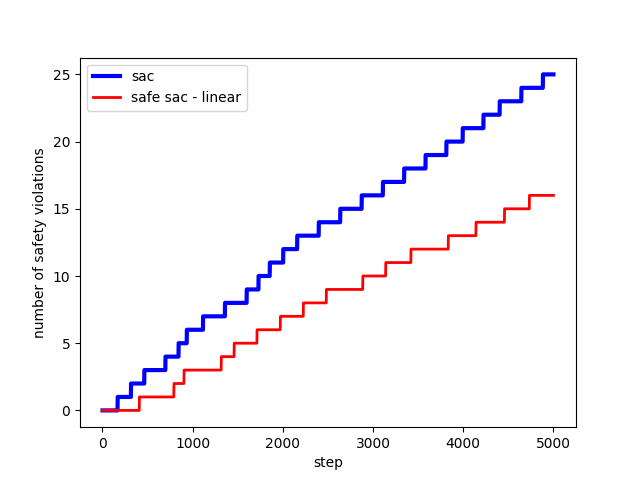
\includegraphics[width=\textwidth]{fig7b_l_vio.png}
\caption{}
\label{fig:gull}
\end{subfigure}%

\begin{subfigure}[b]{0.45\textwidth}
\centering
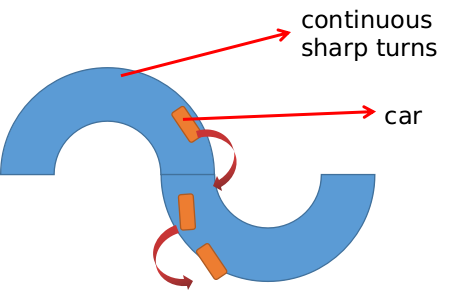
\includegraphics[width=\textwidth]{fig7c_sharp_turns.png}
\caption{}
\label{fig:gull}
\end{subfigure}%
\caption{Comparison of the RL training process with/without safety layer for complicated environment. (a) Discounted reward. (b) Number of violations. (c) A schematic view of continuous sharp turns.}
\end{figure}

We tried to introduce more complicated model to describe the relation between the safety signal and the state/action pairs. Currently only linear approximation is used. Here we try to introduce the quadratic approximation.

$$c(s') \approx c(s) + g_1(s, w_1)^\intercal a + \frac{1}{2} a^\intercal g_2(s, w_2) a$$
\begin{equation}
arg \min_{w_1, w_2} \quad \sum_{(s, a, s')\in D} (c_i(s') - (c(s) + g_1(s, w_1)^\intercal a + \frac{1}{2} a^\intercal g_2(s, w_2) a)^2\\
\end{equation}

Where $g_1(s, w_1)$ is a vector as described before, and $g_2(s,w_2)$ is a symmetric matrix. Both $g_1$ and $g_2$ are produced by neural networks. Then the safety layer would revise the proposed action according to the following.

\begin{equation}
\begin{aligned}
arg \min_{a} \quad & \frac{1}{2} |a - \mu_{\theta}(s)|^2\\
\textrm{s.t.} \quad & c(s) + g_1(s, w_1)^\intercal a + \frac{1}{2} a^\intercal g_2(s, w_2) a \leq C_{critical}\\
\end{aligned}
\end{equation} 

Equation 8 is a quadratic constrained quadratic programming (QCQP) problem. Unfortunately there are no close form solutions to the QCQP problem. Here we use some heuristics to solve this problem, such as \cite{park2017general}. Basically each time the current policy proposes the action, we solve Equation 8 with QCQP solver \cite{park2017general} to get the revised action and then apply it to the car. The QCQP problem might not always be solvable. In case of failures from the solver, we take the originally proposed action. We have tried this quadratic approximation for safety layer for our complicated environment. However, it does not work. The results are shown in Figure 8.

\begin{figure}[ht]
\centering
\begin{subfigure}[b]{0.45\textwidth}
\centering
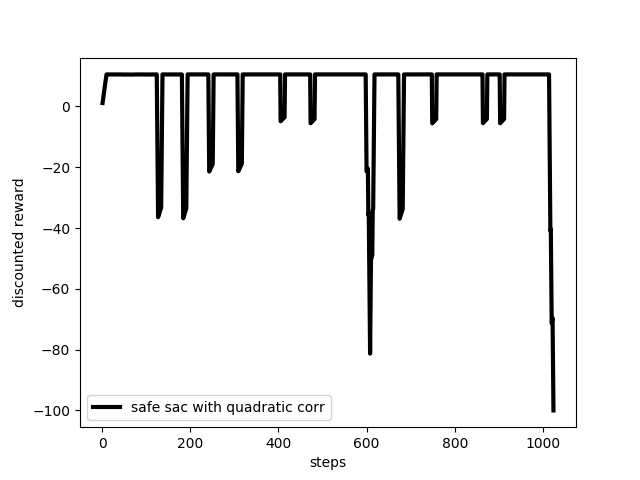
\includegraphics[width=\textwidth]{fig8a_q_reward.png}
\caption{}
\label{fig:gull}
\end{subfigure}%
\begin{subfigure}[b]{0.34\textwidth}
\centering
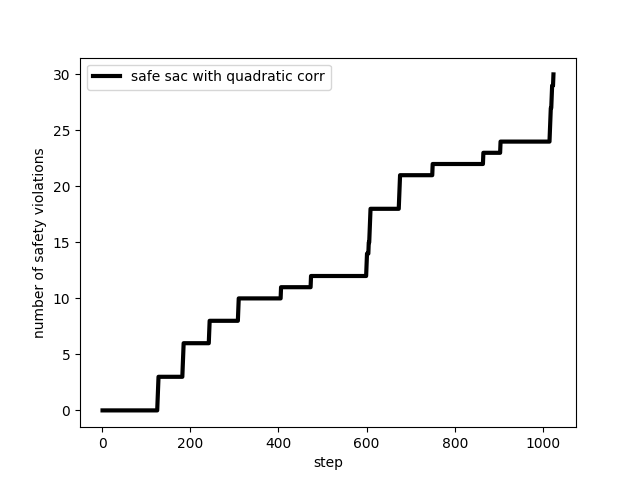
\includegraphics[width=\textwidth]{fig8b_q_vio.png}
\caption{}
\label{fig:gull}
\end{subfigure}%
\caption{Comparison of the RL training process with/without safety layer (quadratic approximation) for complicated environment. (a) Discounted reward. (b) Number of violations.}
\end{figure}


Figure 8 shows that with the quadratic approximation of the safety layer, the performance becomes even worse than the non-safety-layer case. This shows that under current setup, more complicated approximation for the safety signals would not enhance the performance, since it brings new trouble (e.g. QCQP not solvable). More energies should be spent on the RL algorithm itself, for instance, redesign the reward function to reduce the impact of current speed, so that the learned policy would not drive the car too fast, in order to take in-time actions to avoid safety violations with sudden appearance of sharp turns.
%===============================================================================================================

\section{Conclusion}
In this project, we implement the linearly approximated safety layer method proposed by \cite{dalal2018safe} to investigate its effect on autonomous drive applications. Concerning simple environment, the method does bring in much fewer safety violations (although still not zero violations). When it comes to complicated environment, the RL training process with safety layer still has many safety violations, although fewer than the case without the safety layer. We then bring in the quadratic approximation for the safety layer, only to see it makes the performance even worse.

Looks like the proposed simple safety layer method still has some issues when applied to RL problems with complicated environments. The safety guarantee at the inital stage of the RL process still remains an open questions. More considerations should be laid concerning design of the RL algorithm and the correction of the proposed actions to produce a general enough approach for safety guarantees.


\bibliography{iclr2018_conference}
\bibliographystyle{iclr2018_conference}

\end{document}
